
To better understand how coordination facts are used, we next present some programs that
take advantage of them.

\subsection{Single Source Shortest Path}

The Single Source Shortest Path (SSSP) program was already presented in
Section~\ref{sec:language}. We are going to update the code in
Fig.~\ref{code:shortest_path_program} so that nodes with the shortest distances
are selected to run before others nodes. The coordinated version of the same
algorithm is presented in Fig.~\ref{code:shortest_path_program_coord} and it
uses one coordination fact, namely \texttt{set-priority} (line 15). Note that we
also use a global program directive to order priorities in ascending order (line
5).

When using a single thread, the algorithm behaves like
Dijkstra's shortest path algorithm~\cite{Dijkstra}. However, when using multiple
threads, each thread will pick the smallest distance from their subset of nodes.
While this is not optimal since threads do not share a global view of priorities,
many rule derivations are going to be avoided.

\begin{figure}[h!]
\scriptsize\begin{Verbatim}[numbers=left,commandchars=\\\{\}]
type route edge(node, node, int).
type linear shortest(node, int, list int).
type linear relax(node, int, list int).

\underline{priority @order asc}.

shortest(A, +00, []).
relax(@1, 0, [@1]).

relax(A, D1, P1), shortest(A, D2, P2),
D1 < D2
   -o shortest(A, D1, P1),
      \{B, W | !edge(A, B, W) |
         relax(B, D1 + W, P1 ++ [B]),
         \underline{set-priority(B, float(D1 + W))}\}.

relax(A, D1, P1), shortest(A, D2, P2),
D1 >= D2
   -o shortest(A, D2, P2).
\end{Verbatim}
  \caption{Shortest Path Program.}
  \label{code:shortest_path_program_coord}
\end{figure}
\normalsize

The most interesting property of the SSSP program presented in
Fig.~\ref{code:shortest_path_program_coord} is that it remains provably correct,
although it applies rules using smarter ordering. The derivation of
\texttt{set-priority} does not change the behavior of the logical rules and the
code remains declarative.

Figure~\ref{results:sssp_uspowergrid} shows experimental results for a variant of
the SSSP program that computes the SSSP for many of the nodes of the graph.
There are some situations where unecessary facts are propagated
because although the shortest distance is selected, sub-optimal distances may be
propagated because many SSSP distances are computed at the same time.
However, we see a reduction of over 50\% in the number of
derived facts when using the coordinated version \textbf{C} over the regular
version \textbf{R}. The results also show that the cordinated
version using 16 threads is 1.3 times faster than the regular version using 16
threads. In turn, this makes the coordinated version 20 times faster
than the regular version using 1 thread.

\begin{figure}[h!]
   \begin{center}
      \subfloat[]{ \begin{tabular}[b]{ | c | c | c | }
         \hline                       
         \textbf{\# T} & \textbf{R} & \textbf{C} \\ \hline \hline
         1 & 333K & 206K \\
         2 & 300K & 210K \\
         4 & 316K & 208K \\
         8 & 328K & 211K \\
         16 & 343K & 212K \\
         \hline  
         \end{tabular}
         \normalsize
      }
      \subfloat[]{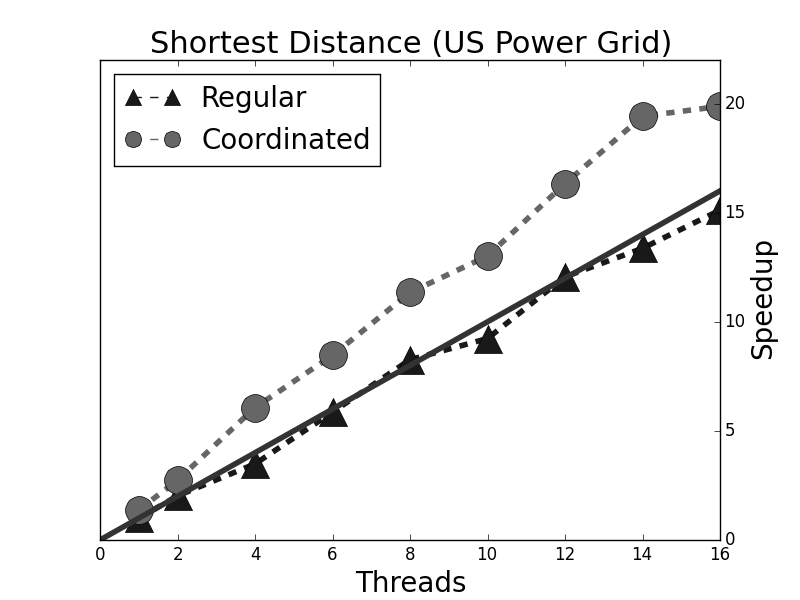
\includegraphics[width=5cm]{results/shortest-uspowergrid.png}}
   \end{center}
   \caption{Experimental results for the SSSP program using US powergrid network.
   On the left we show the number of facts derived for the regular \textbf{R}
   and coordinated version \textbf{C} using a variable number of threads
   \textbf{\# T}. On the right, we have the scalability of the regular version
   and coordinated version. The speedup values are computed using the execution
   time of the regular version for 1 thread.}
   \label{results:sssp_uspowergrid}
\end{figure}

\subsection{MiniMax}

The MiniMax algorithm is a decision rule algorithm for minimizing the
possible loss for a worst case (maximum loss) scenario in a zero sum
game for 2 (or more) players that play in
turns~\cite{Edwards54}.

The algorithm proceeds by building a game tree, where each tree node represents a
game state and the children represent the possible game moves that can
be made by either player 1 or player 2. The
tree levels are built in a way that each player plays in turns and the
first level represents the moves made by player 1.  An
evaluation function \texttt{f(State)} is used to compute the score of
the board for each leaf of the tree. A node is a leaf when it can no longer be
expanded since the state represents a possible end of the game.  Finally, the
algorithm recursively minimizes or maximizes the scores of each node.
To select the best move for player 1, the
algorithm picks the move maximized at the root node.

In LM, the program starts with a root node (with the initial game state)
that is expanded with the available moves at each level. The graph of the
program is dynamic since nodes are created and eventually deleted once they
have nore more facts or no more references to them. The latter happens when the
leaves scores are computed or when a node fully minimizes or maximizes the
children scores. When the program ends, only the root node is have facts in its
database.

The LM code in Fig.~\ref{minimax:check-end} implements
the initial expansion of the tree. The first three rules (lines 1-10) deal
with the cases where no children nodes are created and the last three rules
(12-29) deal with cases where new nodes may be created.
Thes rule in lines 12-25 generate new nodes using the
\texttt{exists} language construct, which creates a new node address
\texttt{B}, where a new \texttt{play} fact is created with the new
board. A \texttt{parent(B,A)} fact is derived to allow node \texttt{B} to
communicate with its parent.

Since our implementation
uses a FIFO ordering for nodes, meaning that when children are expanded, we
first expand each children and then the children of the children. The default
ordering of the system works well enough for most practical purposes. We note
however, that this is not optimal for this program since the complete tree needs
to be expanded before computing the scores at the leaves. This introduces memory
issues since, in the worst case, the memory needs of the program are
$\mathcal{O}(n)$, where $n$ is the number of nodes in the tree.

\begin{figure}[h!]
\scriptsize\begin{Verbatim}[numbers=left,commandchars=\\\{\}]
expand(A, Board, [], 0, P, \underline{Depth})
  -o leaf(A, Board).

expand(A, Board, [], N, P, \underline{Depth}),
N > 0
  -o maximize(A, N, -00, 0).

expand(A, Board, [], N, P, \underline{Depth}),
N > 0, NextPlayer <> RootPlayer
  -o minimize(A, N, +00, 0).

expand(A, Board, [0 | Xs], N, P, Depth),
Depth >= 5
  -o exists B. (\underline{set-static(B)},
       \underline{set-default-priority(B, float(Depth + 1))},
       play(B, Board ++ [P | Xs], next(P), \underline{Depth + 1}),
       expand(A, Board ++ [0], Xs, N + 1, P, \underline{Depth}),
       parent(B, A)).

expand(A, Board, [0 | Xs], N, P, Depth),
Depth < 5
  -o exists B. (\underline{set-default-priority(B, float(Depth + 1))},
       play(B, Board ++ [P | Xs], next(P), \underline{Depth + 1}),
       expand(A, Board ++ [0], Xs, N + 1, P, \underline{Depth}),
       parent(B, A)).

expand(A, Board, [C | Xs], N, P, \underline{Depth})
C <> 0
  -o expand(A, Board ++ [C], Xs, N, P, \underline{Depth}).
\end{Verbatim}
\caption{MiniMax: checking if the game has ended and expanding the tree}
\label{minimax:check-end}
\end{figure}
\normalsize

With coordination, we set the priority nodes to be the same as the
depth so that the tree is expanded in a depth-first fashion (lines 15 and 22).
The memory complexity of the program then becomes $\mathcal{O}(d t)$, where $d$
is the depth of the tree and $t$ is the number of threads. In
Fig.~\ref{fig:minimax}, we have two threads (squares) and the first one has
expanded the tree on the left side. When a second thread comes up, it steals the
first unexpanded node and expands the tree from that position. Since threads
prioritize deeper nodes, the scores of the first leaves are immediatelly
computed and then sent to the parent node. At this point, the leaves are deleted
and reused for other nodes in the tree, resulting in minimal memory usage.

\begin{figure}[h!]
   \begin{center}
      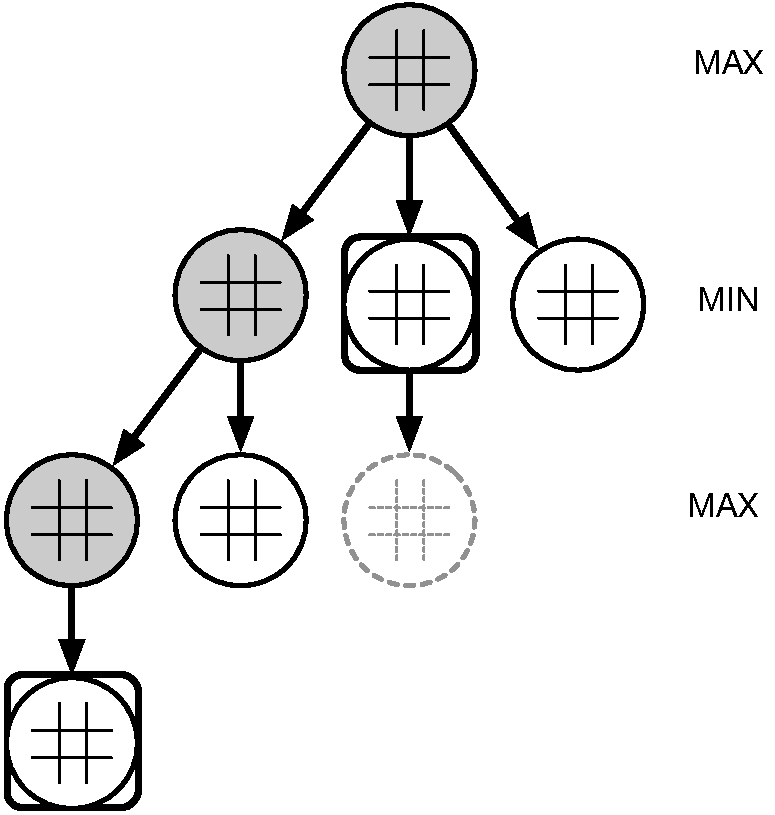
\includegraphics[width=4.5cm]{figures/minimax_tree}
   \end{center}
   \caption{Expanding the MiniMax tree using coordination. By prioritizing
      deeper nodes, threads are forced to expand the tree using a depth-first
      approach, which is superior since there is no need to expand the whole
      tree before computing the node scores.}
   \label{fig:minimax}
\end{figure}

We also take advantage of memory locality by using \texttt{set-static} (line
14), so that nodes after a certain level are not stolen by other threads. While
this is not critical for performance in shared memory systems where node
stealing is fairly efficient, we expect that such coordination to be critical in
distributed systems.

\subsection{Heat Transfer}

\subsection{Splash BP}

Randomized and approximation
algorithms can obtain significant benefits from coordination directives because although the final
program results will not be exact, they follow important statistical properties and can be computed faster.
Examples of such programs are PageRank~\cite{Lubachevsky:1986:CAA:4904.4801} and
Loopy Belief Propagation~\cite{Gonzalez+al:aistats09paraml}.

Loopy Belief Propagation~\cite{Murphy99loopybelief} (LBP) is an approximate inference algorithm
used in graphical models with cycles. In its essence, LBP is a sum-product message passing algorithm
where nodes exchange messages with their immediate neighbors and apply some computations to the messages
received.

LBP is an algorithm that maps very well to the graph based model of LM. In its original form, we need to compute
the belief of all nodes for several iterations and also synchronize after each iteration.
However, it is still possible to apply
some optimizations in order to take advantage of the fact that LBP will converge even when using
an asynchronous approach. So, instead of computing the belief iteratively,
we first keep track of all messages sent/received (and overwrite them when we receive a new one)
and recompute the belief when we want, instead of synchronizing between nodes.
This way, we can prioritize the computation of beliefs when
a node's belief value changes significantly. When that happens, we set the priority of its
neighbors so that they can recompute their beliefs.

The asynchronous approach proves to be a nice improvement over the synchronous version. Still, it
is possible to do even better. Gonzalez et al~\cite{Gonzalez+al:aistats09paraml} developed an optimal
algorithm to compute this algorithm by first building a tree and then updating the beliefs of each node twice, first from the leaves to the root and then from the root to the leaves. The root of this tree
is the node with the highest priority (based on belief) while the other nodes in the tree
must have a non-zero priority. Note that the priorities are updated whenever a neighbor updates
their belief. These splash trees are built iteratively until we reach convergence.

\begin{figure}[h!]
   \begin{center}
      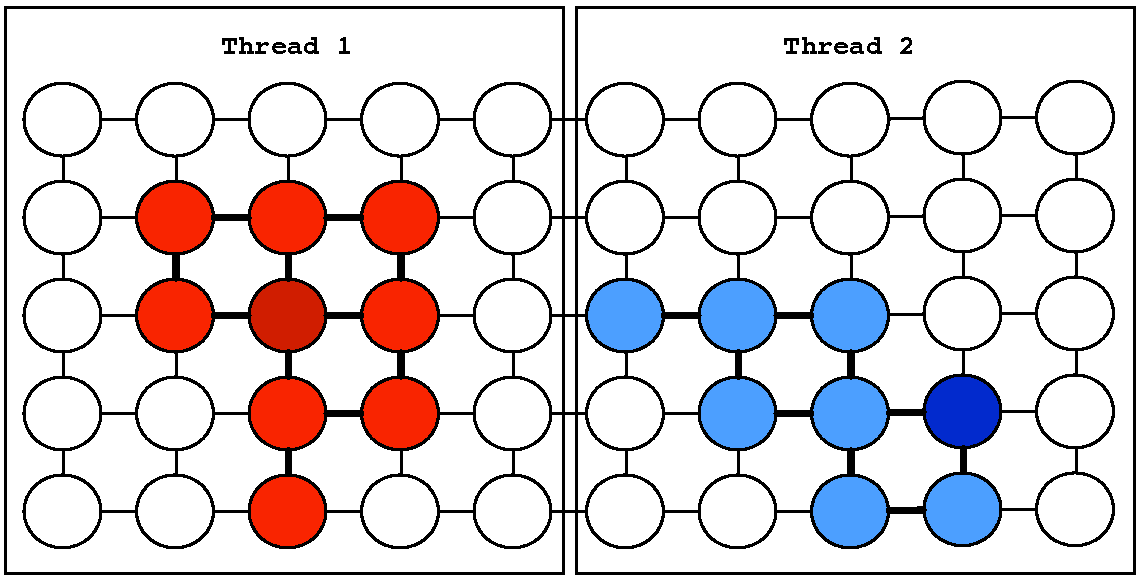
\includegraphics[width=6.5cm]{figures/splash_bp}
   \end{center}
   \caption{Single Source Shortest Path program code.}
   \label{splash_bp}
\end{figure}


The code in Fig.~\ref{code:sbp} presents the coordination code of the Belief Propagation problem.
Please note that we just appended the code in Fig.~\ref{code:sbp} to a working but
unoptimized version of the algorithm.
In the coordination code we have three sections:
\begin{description}
   \item[Tree building]: Each node has a \texttt{waiting} fact that is used to start the tree building process. When the highest priority is picked we create a token that will navigate through the tree. Note that in the rule located in lines 11-18 we check if the priority of the new node to add to the tree is positive and that both nodes are in the same thread. We want the tree to be kept in the same thread.
   \item[First phase]: In the third rule (lines 8-9), when we reach a certain number of nodes in the tree, we generate \texttt{first-phase} in order to update the beliefs of all nodes in tree starting from the leaves and ending at the root. As we update the nodes, we generate \texttt{update} to update the belief values (line 29).
   \item[Second phase]: In the second phase we go from the root to the leaves and update the beliefs a second time (line 39).
\end{description}

When we have several threads, every thread will generate their own trees by taking into account the highest priority node in their own queues.

\begin{figure}[h!]
\scriptsize\begin{Verbatim}[numbers=left,commandchars=*\{\}]
set-static(A). // all nodes are static.

// TREE BUILDING
// continue tree
waiting(A), token(A, All, Next) -o token(A, All, Next).
// start tree
waiting(A), *underline{@priority(A, A, P)}, P > 0.0
   -o token(A, [A], [A]).
// end tree building
token(A, All, Next), length(All) > maxnodes
   -o first-phase(A, All, reverse(All)).
// expand tree
token(A, All, [A | Next])
   -o [collect => L | Side | !edge(A, L, Side),
         0 = count(All, L),
         0 = count(Next, L),
         *underline{priority(A, L, P)}, P > 0.0,
         *underline{cpu-id(A, L, Id1)},
         *underline{cpu-id(A, A, Id2)}, Id1 = Id2 |
         send-token(A, All, Next ++ L)].

send-token(A, All, [])
   -o first-phase(A, All, reverse(All)).
send-token(A, All, [B | Next])
   -o *underline{schedule-next(B)},
      token(B, All ++ [B], [B | Next]).

// FIRST PHASE
first-phase(A, [A], [A]) -o second-phase(A, [], A).
first-phase(A, [A, B | Next], [A])
   -o update(A), *underline{schedule-next(B)},
      second-phase(B, [B | Next], A).
first-phase(A, All, [A, B | Next])
   -o update(A), *underline{schedule-next(B)},
      first-phase(B, All, [B | Next]).

// SECOND PHASE
second-phase(A, [], _)
   -o *underline{set-priority(A, 0.0)}, waiting(A), update(A).
second-phase(A, [A], Back)
   -o update(A), waiting(Back),
      waiting(A), *underline{set-priority(A, 0.0)}.
second-phase(A, [A, B | Next], Back)
   -o update(A), waiting(Back), *underline{schedule-next(B)},
      second-phase(B, [B | Next], A).
\end{Verbatim}
  \caption{Coordination code for the Splash Belief Propagation program.}
  \label{code:sbp}
\end{figure}
\normalsize
